% Keeps the native STATADIC PGFplots closure in the vendored bundle even before a
% project adopts it. The fragment matches PlotSpec.to_pgfplots output.
\documentclass[11pt]{article}
\usepackage{booktabs}
\usepackage{pgfplots}
\pgfplotsset{compat=1.18}
\pagestyle{empty}
\begin{document}
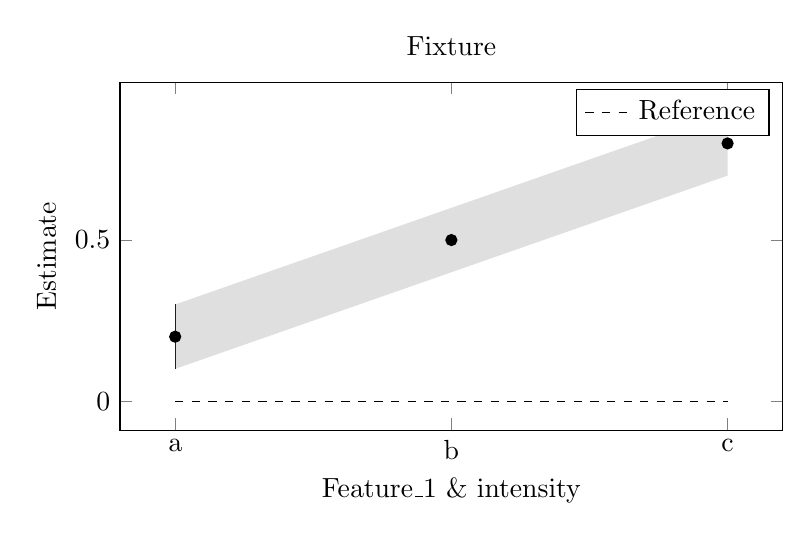
\begin{tikzpicture}
  \begin{axis}[width=10cm,height=6cm,xlabel={Feature\_1 \& intensity},ylabel={Estimate},title={Fixture},xtick={1,2,3},xticklabels={{a},{b},{c}}]
    \addplot[no marks,forget plot] coordinates {(1,0.1) (1,0.3)};
    \addplot[only marks,forget plot] coordinates {(1,0.2) (2,0.5) (3,0.8)};
    \addplot[draw=none,fill=gray,fill opacity=0.25,forget plot] coordinates {(1,0.1) (3,0.7) (3,0.9) (1,0.3)} -- cycle;
    \addplot[dashed,no marks] coordinates {(1,0) (3,0)};
    \addlegendentry{Reference}
  \end{axis}
\end{tikzpicture}
\end{document}
